\documentclass[11pt,a4paper]{article}

\usepackage{kotex}
\usepackage{amsmath,amssymb,mathtools}
\usepackage{geometry}
\usepackage{graphicx}
\usepackage{booktabs}
\usepackage{longtable}
\usepackage{tabularx}
\usepackage{array}
\usepackage{enumitem}
\usepackage{xcolor}
\usepackage{hyperref}
\usepackage{url}
\usepackage{tikz}
\usepackage{pdflscape}
\usetikzlibrary{arrows.meta,positioning,calc,matrix,fit,shapes.geometric}

\geometry{margin=22mm}
\hypersetup{
  colorlinks=true,
  linkcolor=blue!50!black,
  citecolor=blue!50!black,
  urlcolor=blue!50!black
}
\setlist[itemize]{topsep=3pt,itemsep=2pt,parsep=0pt,leftmargin=1.5em}
\setlist[enumerate]{topsep=3pt,itemsep=2pt,parsep=0pt,leftmargin=1.6em}
\renewcommand{\arraystretch}{1.22}
\emergencystretch=2em

\definecolor{ink}{HTML}{0F172A}
\definecolor{muted}{HTML}{475569}
\definecolor{linegray}{HTML}{CBD5E1}
\definecolor{softblue}{HTML}{E0F2FE}
\definecolor{softgreen}{HTML}{DCFCE7}
\definecolor{softorange}{HTML}{FFEDD5}
\definecolor{softred}{HTML}{FEE2E2}
\definecolor{softpurple}{HTML}{F3E8FF}
\definecolor{softyellow}{HTML}{FEF9C3}
\definecolor{blueaccent}{HTML}{2563EB}
\definecolor{greenaccent}{HTML}{16A34A}
\definecolor{orangeaccent}{HTML}{EA580C}
\definecolor{redaccent}{HTML}{DC2626}
\definecolor{purpleaccent}{HTML}{7C3AED}
\definecolor{yellowaccent}{HTML}{CA8A04}

\newcolumntype{Y}{>{\raggedright\arraybackslash}X}
\newcommand{\R}{\mathbb{R}}
\newcommand{\SO}{\mathrm{SO}(3)}
\newcommand{\SE}{\mathrm{SE}(3)}
\newcommand{\norm}[1]{\left\lVert #1 \right\rVert}
\newcommand{\code}[1]{\texttt{#1}}
\newcommand{\paper}[1]{\textit{#1}}
\newcommand{\score}[1]{\textbf{#1}}

\tikzset{
  block/.style={draw, rounded corners=2pt, align=center, inner sep=4pt, font=\small},
  bblue/.style={block, fill=softblue, draw=blueaccent!70!black},
  bgreen/.style={block, fill=softgreen, draw=greenaccent!70!black},
  borange/.style={block, fill=softorange, draw=orangeaccent!70!black},
  bred/.style={block, fill=softred, draw=redaccent!70!black},
  bpurple/.style={block, fill=softpurple, draw=purpleaccent!70!black},
  byellow/.style={block, fill=softyellow, draw=yellowaccent!70!black},
  smallblock/.style={block, font=\scriptsize, minimum height=8mm, text width=24mm},
  var/.style={circle, draw=blueaccent!70!black, fill=softblue, align=center, font=\scriptsize, minimum size=9mm},
  factor/.style={rectangle, rounded corners=1pt, draw=orangeaccent!70!black, fill=softorange, align=center, font=\scriptsize, minimum width=12mm, minimum height=7mm},
  obs/.style={circle, draw=greenaccent!70!black, fill=softgreen, align=center, font=\scriptsize, minimum size=8mm},
  risk/.style={diamond, aspect=1.75, draw=redaccent!70!black, fill=softred, align=center, font=\scriptsize, inner sep=1.6pt},
  arrow/.style={-{Latex[length=2.1mm]}, thick},
  dashedarrow/.style={-{Latex[length=2.1mm]}, thick, dashed},
  axis/.style={draw=linegray, line width=0.35pt},
  heatHigh/.style={fill=softgreen, draw=greenaccent!60!black, rounded corners=1pt, align=center, font=\scriptsize},
  heatMed/.style={fill=softyellow, draw=yellowaccent!60!black, rounded corners=1pt, align=center, font=\scriptsize},
  heatLow/.style={fill=softred, draw=redaccent!60!black, rounded corners=1pt, align=center, font=\scriptsize},
  heatNA/.style={fill=linegray!35, draw=linegray, rounded corners=1pt, align=center, font=\scriptsize}
}

\title{\textbf{VINS 및 Visual-Inertial SLAM 문헌 분석 리포트}\\
\large 수중 이미지 매칭 및 UUV SLAM 적용 관점의 비판적 비교}
\author{under\_water\_image\_match 프로젝트 문헌 정리}
\date{2026년 5월}

\begin{document}
\maketitle

\begin{abstract}
본 리포트는 VINS-Mono, VINS-Fusion, OKVIS, MSCKF, ORB-SLAM3, OpenVINS, Kimera, 그리고 수중 Visual-Inertial SLAM 계열 논문을 하나의 기술 계보로 정리한다.
분석의 초점은 단순 논문 요약이 아니라, 각 시스템이 어떤 관측 모델과 최적화 구조를 택했는지, 어떤 환경 가정 위에서 성능을 얻었는지, 그리고 수중 UUV 환경에서 무엇이 깨지는지에 둔다.
결론적으로 VINS 계열은 ``카메라-IMU tight coupling + IMU preintegration + sliding-window optimization + marginalization''의 실용적 기준선이다.
하지만 수중에서는 낮은 contrast, scattering, feature dropout, 조명 변화, 느린 motion excitation, scale 관측성 저하 때문에 VINS 단독을 최종 해법으로 삼기 어렵다.
현실적인 연구 방향은 VINS-Fusion 또는 OpenVINS를 baseline으로 두고, learned feature matching, pressure/depth, DVL, sonar, acoustic range factor를 graph에 추가하는 것이다.
\end{abstract}

\tableofcontents
\clearpage

\section{리포트의 관점과 결론}

VINS라는 이름은 문헌에서 두 가지 의미로 쓰인다.
좁은 의미의 VINS는 Qin, Li, Shen의 VINS-Mono와 그 코드 계열을 가리킨다 \cite{qin2018vinsmono}.
넓은 의미의 VINS는 visual-inertial navigation system, 즉 카메라와 IMU를 융합하는 상태 추정 시스템 전체를 의미한다.
본 리포트는 두 의미를 구분한다.
``VINS-Mono'' 또는 ``VINS-Fusion''이라고 쓸 때는 HKUST Aerial Robotics Group의 구현 계열을 의미하고, ``VINS 계열''이라고 쓸 때는 visual-inertial estimation 전체를 의미한다.

\subsection{핵심 판단}

\begin{itemize}
  \item VINS-Mono의 학술적 가치는 완전히 새로운 수학 하나가 아니라, VIO에 필요한 initialization, calibration, failure recovery, loop closure, pose graph를 통합한 \textbf{실전형 monocular visual-inertial estimator}라는 데 있다.
  \item OKVIS는 bounded keyframe window와 nonlinear optimization 기반 VIO의 수학적 기준선이고 \cite{leutenegger2015okvis}, MSCKF는 filter-based VIO의 기준선이다 \cite{mourikis2007msckf}.
  \item IMU preintegration은 VIO backend를 실시간으로 만드는 핵심이며, Forster 등의 on-manifold preintegration 논문이 이 계열의 표준 참고문헌이다 \cite{forster2017preintegration}.
  \item ORB-SLAM3는 VINS-Mono보다 SLAM 시스템성이 강하다. 특히 multi-map, relocalization, map reuse, place recognition 측면에서 비교 기준이 된다 \cite{campos2021orbslam3}.
  \item 수중 환경에서는 vision-only 또는 vision+IMU만으로는 불충분하다. SVIn2, RD-VIO, AQUA-SLAM 등 수중 특화 논문들은 공통적으로 pressure, sonar, DVL, acoustic cue를 factor graph에 추가한다 \cite{rahman2022svin2,li2023rdvio,xu2025aquaslam}.
\end{itemize}

\subsection{수중 프로젝트에 대한 실무적 결론}

현재 \code{under\_water\_image\_match} 프로젝트가 수중 image matching에서 출발한다면, 연구 baseline은 다음 순서가 타당하다.

\begin{enumerate}
  \item 지상/표준 VIO baseline: VINS-Fusion, OpenVINS, ORB-SLAM3.
  \item 수중 영상 frontend: CLAHE, color correction, dehazing, learned feature detector/descriptor, robust optical flow.
  \item 수중 보조 센서: pressure/depth factor를 먼저 넣고, 가능하면 DVL 또는 sonar factor를 추가.
  \item loop closure: BoW만으로 끝내지 말고 NetVLAD, AP-GeM, SuperGlue/LightGlue 기반 geometric verification 등으로 재검토.
  \item 평가 dataset: EuRoC만으로 주장하지 말고 AQUALOC, FLSea, 자체 수중 tank/수영장 sequence를 반드시 포함.
\end{enumerate}

\section{문헌 계보}

Visual-Inertial SLAM의 발전은 크게 세 갈래로 볼 수 있다.
첫째, MSCKF로 대표되는 filtering 계열.
둘째, OKVIS와 VINS-Mono로 대표되는 sliding-window nonlinear optimization 계열.
셋째, ORB-SLAM3와 Kimera처럼 VIO를 SLAM, dense/semantic mapping, multi-map framework로 확장하는 계열이다.

\begin{figure}[htbp]
\centering
\resizebox{\linewidth}{!}{%
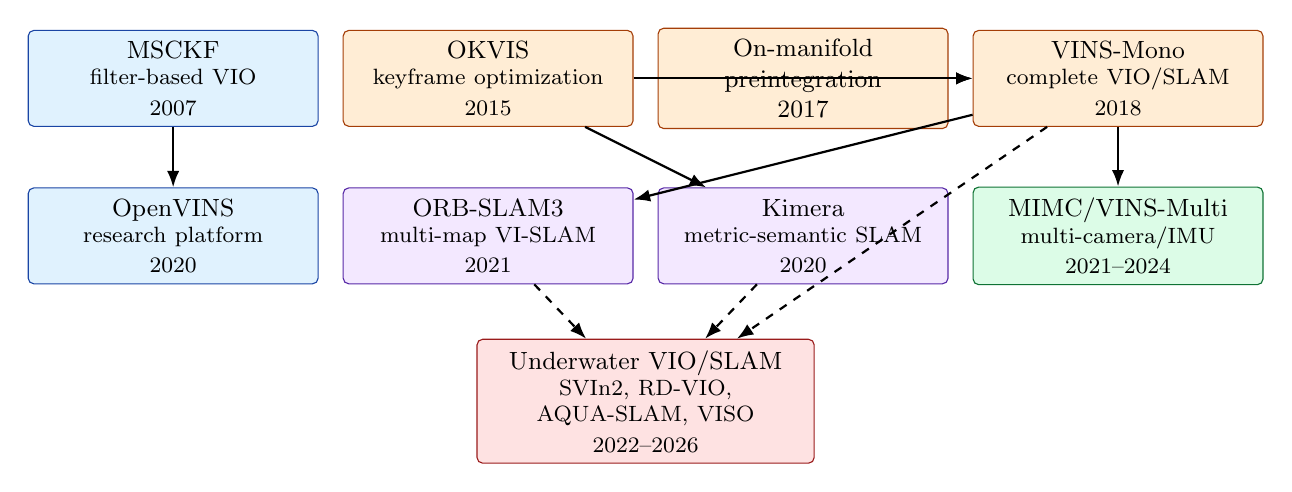
\begin{tikzpicture}[x=1cm,y=1cm]
  \node[bblue, text width=34mm] (msckf) at (0,2.9) {MSCKF\\\footnotesize filter-based VIO\\2007};
  \node[borange, text width=34mm] (okvis) at (4.0,2.9) {OKVIS\\\footnotesize keyframe optimization\\2015};
  \node[borange, text width=34mm] (preint) at (8.0,2.9) {On-manifold\\preintegration\\2017};
  \node[borange, text width=34mm] (vins) at (12.0,2.9) {VINS-Mono\\\footnotesize complete VIO/SLAM\\2018};

  \node[bblue, text width=34mm] (openvins) at (0,0.9) {OpenVINS\\\footnotesize research platform\\2020};
  \node[bpurple, text width=34mm] (orb3) at (4.0,0.9) {ORB-SLAM3\\\footnotesize multi-map VI-SLAM\\2021};
  \node[bpurple, text width=34mm] (kimera) at (8.0,0.9) {Kimera\\\footnotesize metric-semantic SLAM\\2020};
  \node[bgreen, text width=34mm] (multi) at (12.0,0.9) {MIMC/VINS-Multi\\\footnotesize multi-camera/IMU\\2021--2024};

  \node[bred, text width=40mm] (under) at (6.0,-1.2) {Underwater VIO/SLAM\\\footnotesize SVIn2, RD-VIO, AQUA-SLAM, VISO\\2022--2026};

  \draw[arrow] (msckf) -- (openvins);
  \draw[arrow] (okvis) -- (vins);
  \draw[arrow] (preint) -- (vins);
  \draw[arrow] (vins) -- (multi);
  \draw[arrow] (okvis) -- (kimera);
  \draw[arrow] (vins) -- (orb3);
  \draw[dashedarrow] (vins) -- (under);
  \draw[dashedarrow] (orb3) -- (under);
  \draw[dashedarrow] (kimera) -- (under);
\end{tikzpicture}}
\caption{Visual-Inertial SLAM 문헌 계보. VINS-Mono는 optimization-based VIO의 실용형 기준선이며, 수중 SLAM은 이 계열에 sonar/depth/DVL/acoustic factor를 추가하는 방향으로 발전하고 있다.}
\end{figure}

\section{공통 수학 구조}

\subsection{상태 변수}

VIO 시스템의 기본 상태는 보통 다음과 같이 잡는다.

\begin{equation}
\mathcal{X}_k =
\left\{
\mathbf{R}_{WB_k},\,
\mathbf{p}_{WB_k},\,
\mathbf{v}_{WB_k},\,
\mathbf{b}_{a,k},\,
\mathbf{b}_{g,k}
\right\},
\end{equation}

여기서 \(\mathbf{R}_{WB_k}\in\SO\)는 body frame에서 world frame으로의 회전, \(\mathbf{p}_{WB_k}\in\R^3\)는 위치, \(\mathbf{v}_{WB_k}\in\R^3\)는 속도, \(\mathbf{b}_{a,k}\), \(\mathbf{b}_{g,k}\)는 accelerometer 및 gyroscope bias다.
VINS-Mono와 OKVIS 같은 optimization 방식은 sliding window 안의 여러 pose와 landmark inverse depth를 함께 최적화한다.
MSCKF는 landmark를 state에 오래 유지하지 않고, 여러 camera pose가 동일 landmark를 관측한다는 constraint를 measurement update로 사용한다.

\subsection{최적화 문제}

Optimization-based VIO의 backend는 다음 MAP 문제로 볼 수 있다.

\begin{equation}
\min_{\mathcal{X},\mathcal{L}}
\left(
\sum_{(i,j)\in\mathcal{V}}
\norm{\mathbf{r}^{v}_{ij}}^2_{\mathbf{\Sigma}^{-1}_{v}}
+
\sum_{(i,i+1)\in\mathcal{I}}
\norm{\mathbf{r}^{imu}_{i,i+1}}^2_{\mathbf{\Sigma}^{-1}_{imu}}
+
\norm{\mathbf{r}^{prior}}^2_{\mathbf{\Sigma}^{-1}_{prior}}
\right).
\end{equation}

첫 번째 항은 feature reprojection residual, 두 번째 항은 IMU preintegration residual, 세 번째 항은 marginalization으로 얻은 prior residual이다.
Loop closure가 들어가면 pose graph residual이 추가되고, 수중 시스템에서는 pressure, depth, DVL, sonar, acoustic range residual이 더해진다.

\begin{figure}[htbp]
\centering
\resizebox{0.92\linewidth}{!}{%
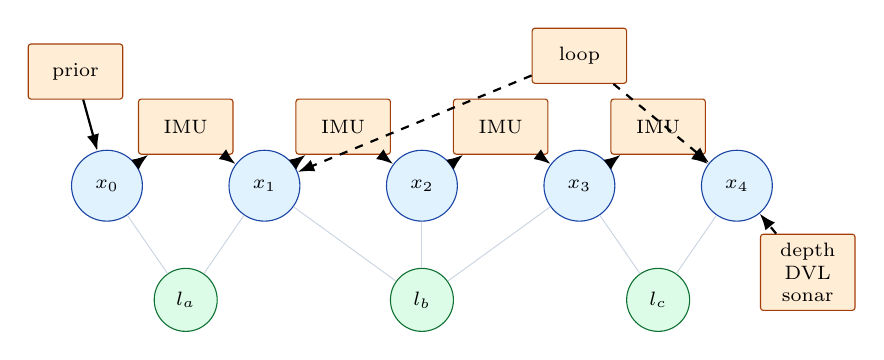
\begin{tikzpicture}[x=1cm,y=1cm]
  \node[var] (x0) at (0,0) {\(x_0\)};
  \node[var] (x1) at (2,0) {\(x_1\)};
  \node[var] (x2) at (4,0) {\(x_2\)};
  \node[var] (x3) at (6,0) {\(x_3\)};
  \node[var] (x4) at (8,0) {\(x_4\)};

  \node[factor] (imu01) at (1,0.75) {IMU};
  \node[factor] (imu12) at (3,0.75) {IMU};
  \node[factor] (imu23) at (5,0.75) {IMU};
  \node[factor] (imu34) at (7,0.75) {IMU};

  \node[obs] (l0) at (1,-1.45) {\(l_a\)};
  \node[obs] (l1) at (4,-1.45) {\(l_b\)};
  \node[obs] (l2) at (7,-1.45) {\(l_c\)};

  \node[factor] (p0) at (-0.4,1.45) {prior};
  \node[factor] (loop) at (6.0,1.65) {loop};
  \node[factor] (depth) at (8.9,-1.10) {depth\\DVL\\sonar};

  \draw[arrow] (x0) -- (imu01);
  \draw[arrow] (imu01) -- (x1);
  \draw[arrow] (x1) -- (imu12);
  \draw[arrow] (imu12) -- (x2);
  \draw[arrow] (x2) -- (imu23);
  \draw[arrow] (imu23) -- (x3);
  \draw[arrow] (x3) -- (imu34);
  \draw[arrow] (imu34) -- (x4);

  \draw[axis] (x0) -- (l0);
  \draw[axis] (x1) -- (l0);
  \draw[axis] (x1) -- (l1);
  \draw[axis] (x2) -- (l1);
  \draw[axis] (x3) -- (l1);
  \draw[axis] (x3) -- (l2);
  \draw[axis] (x4) -- (l2);
  \draw[dashedarrow] (loop) -- (x1);
  \draw[dashedarrow] (loop) -- (x4);
  \draw[dashedarrow] (depth) -- (x4);
  \draw[arrow] (p0) -- (x0);
\end{tikzpicture}}
\caption{Sliding-window VIO factor graph의 개념도. 파란 노드는 pose/velocity/bias 상태, 초록 노드는 landmark, 주황 노드는 residual factor다. 수중 시스템은 depth, pressure, DVL, sonar factor를 추가하여 vision dropout과 scale drift를 보완한다.}
\end{figure}

\subsection{IMU preintegration의 의미}

IMU는 수백 Hz 이상으로 들어오고 영상은 보통 10--30 Hz로 들어온다.
모든 IMU sample을 매번 최적화 변수와 직접 연결하면 계산량이 커진다.
Preintegration은 두 keyframe 사이의 많은 IMU sample을 하나의 relative motion constraint로 압축한다 \cite{forster2017preintegration}.

\begin{align}
\Delta \mathbf{R}_{ij} &\approx \prod_{k=i}^{j-1}
\exp\left((\tilde{\boldsymbol{\omega}}_k-\mathbf{b}_{g,k})\Delta t\right), \\
\Delta \mathbf{v}_{ij} &\approx \sum_{k=i}^{j-1}
\Delta \mathbf{R}_{ik}(\tilde{\mathbf{a}}_k-\mathbf{b}_{a,k})\Delta t, \\
\Delta \mathbf{p}_{ij} &\approx \sum_{k=i}^{j-1}
\left(\Delta \mathbf{v}_{ik}\Delta t
+ \frac{1}{2}\Delta \mathbf{R}_{ik}(\tilde{\mathbf{a}}_k-\mathbf{b}_{a,k})\Delta t^2\right).
\end{align}

중요한 점은 rotation이 Euclidean vector space가 아니라 manifold 위에 있다는 것이다.
따라서 단순 적분보다 \(\SO\) 위의 perturbation, bias correction, covariance propagation을 일관되게 처리해야 한다.
VINS-Mono와 OKVIS의 backend를 이해하려면 이 논문을 기초 문헌으로 삼아야 한다.

\section{핵심 논문별 분석}

\subsection{MSCKF: filter-based VIO의 기준선}

\paper{A Multi-State Constraint Kalman Filter for Vision-Aided Inertial Navigation}은 Extended Kalman Filter 기반 VIO의 대표 논문이다 \cite{mourikis2007msckf}.
핵심 아이디어는 landmark 3D 위치를 filter state에 계속 들고 있지 않고, 동일 feature가 여러 camera pose에서 관측되었다는 geometric constraint만 update에 쓰는 것이다.
이 덕분에 계산량이 feature 수에 대해 상대적으로 잘 제어된다.

\paragraph{기여.}
MSCKF는 대규모 환경에서 실시간 vision-aided inertial navigation을 가능하게 한 고전적 기준선이다.
특히 feature 위치를 state로 오래 유지하지 않는 structureless treatment는 이후 OpenVINS, robocentric VIO, 여러 filter-based VINS 연구의 기반이 되었다.

\paragraph{한계.}
EKF 계열은 linearization point와 consistency에 민감하다.
또한 loop closure와 global map reuse를 자연스럽게 통합하기 어렵다.
수중 환경에서는 feature track이 짧고 outlier가 많아지면 update constraint 자체가 약해진다.
다만 covariance를 명시적으로 얻기 쉽기 때문에, safety-critical navigation이나 sensor health monitoring에는 장점이 있다.

\subsection{OKVIS: optimization-based VIO의 정석}

\paper{Keyframe-Based Visual-Inertial Odometry Using Nonlinear Optimization}은 OKVIS의 핵심 논문이다 \cite{leutenegger2015okvis}.
카메라 reprojection residual과 inertial residual을 probabilistic cost function에 넣고, keyframe window를 marginalization으로 제한하여 실시간성을 확보한다.

\paragraph{기여.}
OKVIS는 VIO를 bundle adjustment와 inertial factor가 결합된 sparse nonlinear least squares 문제로 정식화했다.
이 논문은 ``VIO는 filter로만 해야 한다''는 초기 관성을 깨고, 최적화 기반 접근이 정확도 측면에서 강력하다는 것을 보여주었다.

\paragraph{VINS와의 관계.}
VINS-Mono는 OKVIS류의 sliding-window optimization을 더 실용적인 시스템으로 확장했다.
VINS-Mono에는 robust initialization, failure recovery, loop detection, pose graph optimization, online calibration 같은 engineering layer가 더 강하다.

\paragraph{한계.}
OKVIS 자체는 local VIO 성격이 강하며, full SLAM의 loop closure와 map reuse는 별도 설계가 필요하다.
수중에서는 feature frontend와 calibration이 병목이 된다.

\subsection{On-Manifold Preintegration}

Forster 등의 \paper{On-Manifold Preintegration for Real-Time Visual-Inertial Odometry}는 VIO backend의 핵심 수학을 제공한다 \cite{forster2017preintegration}.
고주파 IMU를 keyframe 사이 relative motion factor로 압축하면서, \(\SO\) manifold 위의 noise와 bias correction을 다룬다.

\paragraph{기여.}
기존 방식은 linearization point가 바뀔 때 IMU를 다시 적분해야 하는 문제가 있었다.
Preintegration은 bias 변화에 대한 first-order correction을 통해 재적분 비용을 크게 줄인다.

\paragraph{비판적 관점.}
Preintegration은 backend 효율을 해결하지만, IMU 자체의 관측성 문제를 해결하지 않는다.
예를 들어 AUV가 천천히 거의 일정한 속도로 움직이면 scale, gravity, accelerometer bias를 분리하기 어렵다.
따라서 수중에서는 depth/pressure/DVL 같은 독립 관측이 필요하다.

\subsection{VINS-Mono}

\paper{VINS-Mono: A Robust and Versatile Monocular Visual-Inertial State Estimator}는 monocular camera와 low-cost IMU를 사용한 complete VIO/SLAM 시스템을 제시한다 \cite{qin2018vinsmono}.
논문은 robust initialization, tightly-coupled nonlinear optimization, IMU preintegration, loop detection, relocalization, 4-DoF pose graph optimization, onboard MAV flight, mobile implementation을 다룬다.

\paragraph{기여.}
VINS-Mono의 가장 큰 기여는 완성도다.
논문 단위의 수식뿐 아니라, 오픈소스 구현을 통해 연구자와 엔지니어가 실제 dataset과 robot에서 바로 검증할 수 있는 기준선을 제공했다.

\paragraph{Backend.}
VINS-Mono backend는 sliding window 안에서 camera pose, velocity, IMU bias, feature inverse depth를 최적화한다.
Visual residual은 normalized image plane의 reprojection error, inertial residual은 preintegrated IMU measurement error다.
Old keyframe은 marginalization되어 prior factor로 남는다.

\paragraph{Frontend.}
VINS-Mono는 KLT optical flow 기반 feature tracking과 RANSAC outlier rejection을 사용한다.
이는 실시간성과 구현 안정성 면에서 좋지만, 수중의 낮은 contrast와 부유물, motion blur, 반복 패턴에서는 쉽게 무너진다.
이 지점이 수중 프로젝트에서 가장 먼저 바꿔야 할 가능성이 큰 부분이다.

\paragraph{Loop closure.}
Loop closure는 local VIO drift를 global consistency로 보정한다.
그러나 place recognition은 appearance stability에 의존한다.
수중에서는 같은 장소라도 조명 각도, 탁도, color attenuation 때문에 descriptor distribution이 크게 바뀐다.
따라서 VINS-Mono의 loop closure를 그대로 수중에 가져가는 것은 위험하다.

\subsection{Online Temporal Calibration}

\paper{Online Temporal Calibration for Monocular Visual-Inertial Systems}는 카메라와 IMU 사이의 time offset을 online optimization 변수로 추정한다 \cite{qin2018temporal}.
실제 hardware에서는 trigger delay, transmission delay, driver timestamp 차이 때문에 sensor timestamp가 정확히 맞지 않는다.

\paragraph{기여.}
VIO 실패의 상당수는 estimator 이론보다 sensor synchronization에서 발생한다.
이 논문은 time offset을 camera/IMU state 및 feature location과 함께 최적화하여 VINS의 실용성을 크게 높였다.

\paragraph{수중 관점.}
수중 vehicle은 cable, embedded computer, camera driver, sonar driver 등으로 timestamp chain이 길어질 수 있다.
따라서 online temporal calibration은 중요하다.
하지만 offset이 관측 가능하려면 충분한 angular/linear excitation이 필요하다.
느리고 단조로운 AUV motion에서는 time offset과 bias/scale이 서로 섞일 수 있다.

\subsection{Relocalization, Global Optimization, Map Merging}

Qin 등의 \paper{Relocalization, Global Optimization and Map Merging for Monocular Visual-Inertial SLAM}은 VINS-Mono 계열을 map reuse와 map merging 방향으로 확장한다 \cite{qin2018relocalization}.
local VIO는 drift가 누적되기 때문에, 이전 map에 relocalize하고 pose graph optimization으로 global consistency를 회복하는 구조가 필요하다.

\paragraph{기여.}
논문은 4-DoF pose graph optimization을 사용한다.
VIO에서 roll/pitch는 gravity로 강하게 제약되지만 yaw와 position drift가 주로 누적된다는 점을 이용한다.
이 판단은 실용적이다.

\paragraph{한계.}
Map reuse는 place recognition이 맞아야 가능하다.
수중에서는 loop candidate retrieval과 geometric verification이 가장 어려운 축에 속한다.
따라서 이 논문은 구조적으로 중요하지만, 수중 적용에는 descriptor와 loop frontend 교체가 필요하다.

\subsection{Visual-Inertial Monocular SLAM with Map Reuse}

Mur-Artal과 Tardos의 \paper{Visual-Inertial Monocular SLAM with Map Reuse}는 ORB-SLAM 계열에서 visual-inertial SLAM과 map reuse를 다룬다 \cite{murartal2017mapreuse}.
VIO가 drift를 누적하는 문제를 loop closure와 map reuse로 해결하려는 관점에서 VINS-Mono relocalization 논문과 비교할 수 있다.

\paragraph{분석.}
이 논문은 visual-inertial odometry보다 SLAM의 map reuse 성격을 더 강하게 강조한다.
이미 mapping된 영역에서 drift-free localization에 가까운 효과를 얻을 수 있다는 점이 핵심이다.
수중 inspection task처럼 같은 구조물을 반복적으로 방문한다면 이 방향이 중요하다.

\subsection{ORB-SLAM3}

\paper{ORB-SLAM3}는 visual, visual-inertial, multi-map SLAM을 통합한 대표 시스템이다 \cite{campos2021orbslam3}.
monocular, stereo, RGB-D, pinhole, fisheye를 지원하고, MAP estimation 기반 visual-inertial SLAM과 multi-map management를 결합한다.

\paragraph{VINS-Mono와의 차이.}
VINS-Mono는 VIO estimator의 완성도가 중심이고, loop closure가 drift 보정 모듈로 붙어 있는 형태에 가깝다.
ORB-SLAM3는 처음부터 SLAM framework, place recognition, map reuse, map merging, atlas를 중심으로 설계되어 있다.

\paragraph{수중 관점.}
장거리 반복 주행이나 구조물 inspection에서는 ORB-SLAM3의 map management가 매력적이다.
그러나 ORB feature와 BoW 기반 place recognition은 수중 영상 변동에 취약할 수 있다.
따라서 ORB-SLAM3 역시 frontend/domain adaptation 없이는 충분하지 않다.

\subsection{OpenVINS}

\paper{OpenVINS}는 VIO 연구 플랫폼이다 \cite{geneva2020openvins}.
on-manifold sliding-window Kalman filter, online intrinsic/extrinsic calibration, time offset calibration, SLAM landmark representation, FEJ treatment, simulator, evaluation toolbox를 제공한다.

\paragraph{기여.}
OpenVINS는 논문 아이디어를 실험 가능한 플랫폼으로 만든 점에서 중요하다.
특히 filter consistency, calibration, uncertainty 추정, simulator 기반 검증에 강하다.

\paragraph{프로젝트 적용성.}
수중 UUV에서는 estimator uncertainty와 sensor degradation을 판단해야 한다.
이 경우 OpenVINS는 VINS-Fusion보다 연구용 diagnostic baseline으로 더 유용할 수 있다.
반대로 loop closure와 full SLAM 기능을 빠르게 쓰려면 VINS-Fusion이나 ORB-SLAM3가 더 편하다.

\subsection{Kimera}

\paper{Kimera}는 real-time metric-semantic SLAM library를 제시한다 \cite{rosinol2020kimera}.
Kimera-VIO, mesh reconstruction, semantic mapping 등으로 확장되는 구조다.

\paragraph{의미.}
Kimera는 VIO가 sparse trajectory estimation에 머물지 않고 dense/semantic map으로 확장되는 방향을 보여준다.
수중 환경에서 navigation만이 아니라 3D reconstruction, inspection, object-level mapping이 목표라면 Kimera 계열의 관점이 중요하다.

\paragraph{한계.}
Semantic mapping은 domain shift에 취약하다.
육상 dataset에서 학습된 segmentation model은 수중 색감, 탁도, 조명 조건에서 일반화가 어렵다.

\subsection{VINS-Fusion}

VINS-Fusion은 VINS-Mono의 코드 계열 확장판으로, mono+IMU, stereo+IMU, stereo-only, GPS fusion 예제를 지원한다 \cite{vinsfusiongithub}.
공식 README는 VINS-Fusion이 VINS-Mono의 extension이며, stereo camera, stereo+IMU, mono+IMU를 지원하고 online spatial/temporal calibration과 visual loop closure를 제공한다고 설명한다.

\paragraph{논문과 코드의 거리.}
VINS-Fusion 자체는 ``paper is not exactly same with code''라고 명시한다.
따라서 학술 인용은 VINS-Mono와 temporal calibration 논문을 중심으로 하고, VINS-Fusion은 실험 baseline 구현으로 다루는 것이 정확하다.

\paragraph{수중 프로젝트에서의 장점.}
Stereo+IMU 구성이 가능하면 monocular scale ambiguity가 줄어든다.
수중에서 pressure/depth sensor를 추가하기 전 단계로 stereo VINS-Fusion을 baseline으로 쓰는 것은 합리적이다.
다만 stereo matching도 물속의 low texture, scattering, refraction, camera housing calibration 문제에 취약하다.

\subsection{MIMC-VINS와 VINS-Multi}

MIMC-VINS는 multiple IMU와 multiple camera를 arbitrary/asynchronous하게 융합하는 VINS estimator를 제안한다 \cite{eckenhoff2021mimcvins}.
VINS-Multi는 asynchronous multi-camera-IMU state estimator로, parallel frontends와 backend optimization을 통해 asynchronous camera frame을 처리한다 \cite{wang2024vinsmulti}.

\paragraph{의미.}
수중 UUV는 전방 카메라, 하방 카메라, stereo rig, sonar, DVL 등 sensor topology가 복잡해질 수 있다.
따라서 단일 카메라-단일 IMU 가정에서 벗어난 multi-sensor asynchronous VINS 문헌은 중요한 확장 방향이다.

\paragraph{한계.}
센서가 많아지면 성능이 자동으로 좋아지는 것이 아니다.
Extrinsic calibration, temporal calibration, observability, failure detection 문제가 더 어려워진다.
수중에서는 장비 mounting 변형, pressure housing, cable delay까지 고려해야 한다.

\section{수중 및 열악 환경 문헌}

\subsection{수중 visual SLAM survey}

\paper{Visual SLAM for underwater vehicles: A survey}는 수중 visual SLAM의 센서, frontend, backend, loop closure, mapping을 체계적으로 정리한다 \cite{yang2022underwatersurvey}.
핵심 메시지는 단순하다.
수중 visual SLAM은 저비용과 풍부한 시각 정보를 제공하지만, particles, light attenuation, scattering, low contrast, dynamic objects 때문에 육상보다 어렵다.

\subsection{SVIn2}

\paper{SVIn2}는 Scanning Profiling Sonar, visual, inertial, water-pressure 정보를 nonlinear optimization framework에서 tight coupling하는 수중 SLAM 시스템이다 \cite{rahman2022svin2}.
논문은 기존 visual 또는 visual-inertial state estimation package들이 수중에서 inaccurate trajectory 또는 complete tracking loss를 보인다고 지적한다.

\paragraph{기여.}
SVIn2의 핵심은 OKVIS류 visual-inertial framework에 acoustic range와 pressure depth를 결합한 것이다.
수중에서는 sonar가 시야 불량에서도 geometry cue를 제공하고, pressure sensor가 vertical drift와 scale refinement를 돕는다.

\paragraph{프로젝트 시사점.}
이 논문은 ``VINS를 수중에 그대로 적용''하는 방향보다 ``VINS/OKVIS backend에 수중 센서 residual을 추가''하는 방향이 정답에 가깝다는 것을 보여준다.

\subsection{RD-VIO}

\paper{RD-VIO: Relative-Depth-Aided Visual-Inertial Odometry for Autonomous Underwater Vehicles}는 monocular VIO의 scale과 initialization 문제를 depth cue로 보완한다 \cite{li2023rdvio}.
AUV의 slow motion과 insufficient excitation은 monocular VIO initialization을 어렵게 만든다.
RD-VIO는 IMU-depth joint initialization과 relative depth residual을 제안한다.

\paragraph{의미.}
수중 vehicle은 MAV처럼 강한 excitation을 만들기 어렵다.
따라서 visual-inertial alignment만으로 scale, gravity, bias를 안정적으로 추정하기 어렵다.
Depth/pressure는 이 문제를 직접 찌르는 강한 보조 관측이다.

\subsection{AQUA-SLAM}

\paper{AQUA-SLAM}은 DVL, stereo camera, IMU를 graph optimization framework에서 tight coupling하고, DVL-camera-IMU extrinsic과 DVL transducer misalignment calibration을 포함한다 \cite{xu2025aquaslam}.

\paragraph{의미.}
수중 SLAM에서 DVL은 매우 강력한 velocity cue다.
그러나 DVL은 calibration 문제가 어렵다.
AQUA-SLAM은 단순히 센서를 추가하는 것이 아니라, calibration을 estimator 설계 안에 넣어야 함을 보여준다.

\subsection{ROFT-VINS}

\paper{ROFT-VINS}는 textureless environment와 illumination change에서 feature tracking을 deep learning으로 강화하고, 이를 VINS-Fusion monocular-inertial pipeline에 통합해 평가한다 \cite{park2026roftvins}.

\paragraph{의미.}
수중 이미지 매칭 프로젝트에 가장 직접적인 시사점은 frontend 교체다.
VINS-Mono/Fusion의 KLT/ORB류 frontend가 깨지는 환경에서는 learned tracking 또는 learned matching을 backend 앞단에 넣어야 한다.

\subsection{VISO와 최근 acoustic/sonar SLAM}

VISO는 stereo camera, IMU, 3D sonar를 융합해 underwater localization과 dense reconstruction을 동시에 목표로 한다 \cite{liu2026viso}.
또 다른 최근 계열은 DVL preintegration, acoustic-depth factors, visual-inertial-acoustic-depth graph를 제안한다 \cite{zhang2025dvlpreintegration}.

\paragraph{비판적 해석.}
최근 수중 SLAM 논문의 공통 방향은 명확하다.
카메라는 texture가 좋을 때 강력하지만 언제든 실패할 수 있으므로, estimator는 camera가 실패할 때도 죽지 않는 sensor graph를 가져야 한다.
수중에서 robust SLAM은 더 좋은 feature 하나만으로 해결되지 않고, sensor redundancy와 failure-aware optimization으로 해결된다.

\section{논문별 비판적 scorecard}

이 절은 각 논문을 ``무엇을 해결했는가''보다 한 단계 더 들어가서, 어떤 가정을 두고 성능을 얻었는지와 수중 UUV 연구에서 무엇을 빌려와야 하는지를 정리한다.
SLAM 논문은 종종 benchmark 수치만으로 비교되지만, 실제 적용에서는 sensor assumption, calibration burden, failure mode가 더 중요하다.

\begin{landscape}
\small
\begin{longtable}{p{29mm}p{34mm}p{38mm}p{42mm}p{42mm}p{44mm}}
\caption{주요 논문별 비판적 scorecard. ``숨은 가정''은 논문이 명시적으로 부정하지는 않지만, 실제 성능을 지탱하는 전제에 가깝다.}\\
\toprule
\textbf{논문/시스템} & \textbf{핵심 질문} & \textbf{방법론적 선택} & \textbf{강한 증거/기여} & \textbf{숨은 가정/취약점} & \textbf{수중 UUV 시사점} \\
\midrule
\endfirsthead
\toprule
\textbf{논문/시스템} & \textbf{핵심 질문} & \textbf{방법론적 선택} & \textbf{강한 증거/기여} & \textbf{숨은 가정/취약점} & \textbf{수중 UUV 시사점} \\
\midrule
\endhead
\bottomrule
\endfoot

MSCKF \cite{mourikis2007msckf}
& Landmark를 state에 넣지 않고도 real-time VIO가 가능한가?
& Multi-state EKF, structureless feature constraint, camera pose clone.
& 계산량과 covariance 관리가 좋고, 이후 filter-based VIO의 기준선이 되었다.
& Linearization point, observability consistency, feature track 품질에 민감하다. Loop closure와 map reuse가 자연스럽지 않다.
& 불확실도 추정과 health monitoring에는 유용하다. 단독 SLAM baseline보다는 estimator diagnostic baseline으로 적합하다. \\

OKVIS \cite{leutenegger2015okvis}
& Visual residual과 inertial residual을 하나의 nonlinear optimization으로 묶으면 정확도가 좋아지는가?
& Keyframe-based sliding window, reprojection error, inertial error, marginalization.
& Optimization-based VIO의 정석을 제공했다. VINS-Mono의 backend 이해에 직접 연결된다.
& Window 밖 정보는 prior로 압축되므로 marginalization linearization 문제가 남는다. Loop/map reuse는 별도 설계가 필요하다.
& 수중 residual 추가의 기본 틀로 좋다. Pressure, DVL, sonar factor를 붙일 때 OKVIS/VINS류 구조가 자연스럽다. \\

Preintegration \cite{forster2017preintegration}
& 고주파 IMU를 factor graph에서 어떻게 효율적으로 다룰 것인가?
& \(\SO\) manifold 위 preintegration, bias correction, covariance propagation.
& 오늘날 optimization-based VIO의 거의 표준 도구가 되었다.
& IMU factor를 효율화할 뿐, scale/bias/gravity 관측성 부족을 해결하지 않는다.
& AUV slow motion에서는 preintegration만으로 충분하지 않다. Depth/DVL factor가 scale과 velocity 관측성을 보강해야 한다. \\

VINS-Mono \cite{qin2018vinsmono}
& Monocular camera와 low-cost IMU로 실전적인 6-DoF state estimation이 가능한가?
& Sliding-window optimization, robust initialization, online calibration, failure recovery, loop closure, 4-DoF pose graph.
& complete open-source VIO/SLAM baseline을 제공했다. MAV flight와 mobile demo까지 포함해 실용성을 보였다.
& KLT/feature frontend, visual loop closure, camera-IMU calibration 품질에 강하게 의존한다.
& baseline으로 훌륭하지만 수중 최종해법은 아니다. Frontend와 sensor factor를 교체/확장하는 출발점으로 써야 한다. \\

Temporal calibration \cite{qin2018temporal}
& Camera와 IMU timestamp offset을 online으로 보정할 수 있는가?
& Time offset을 state variable로 두고 camera/IMU state, feature와 함께 최적화.
& 실제 VIO 실패 원인 중 하나인 time sync 문제를 estimator 안으로 가져왔다.
& 충분한 motion excitation이 있어야 time offset이 관측 가능하다. Offset이 bias/scale과 혼동될 수 있다.
& 수중 로봇의 driver/cable/sensor delay를 고려하면 필수적이다. 다만 느린 motion에서는 별도 calibration sequence가 필요하다. \\

VINS relocalization/map merge \cite{qin2018relocalization}
& Local VIO drift를 map reuse와 pose graph로 줄일 수 있는가?
& Relocalization, 4-DoF pose graph, previous map loading/merging.
& VINS-Mono를 odometry에서 SLAM에 가깝게 끌어올렸다.
& Place recognition이 실패하면 전체 구조가 약해진다. Appearance 변화가 큰 환경에는 취약하다.
& 수중에서는 BoW loop closure를 그대로 믿기 어렵다. Learned/global descriptor와 acoustic/depth consistency check가 필요하다. \\

ORB-SLAM3 \cite{campos2021orbslam3}
& Visual, visual-inertial, multi-map SLAM을 하나의 open-source framework로 통합할 수 있는가?
& MAP estimation, ORB feature, place recognition, atlas/multi-map, BA.
& SLAM framework 완성도가 높고 relocalization/map reuse가 강하다.
& ORB feature와 BoW가 appearance variation에 취약하다. IMU-camera calibration 요구도 높다.
& 반복 방문 inspection에는 좋은 비교군이다. 수중에서는 feature/descriptor domain adaptation 없이는 취약하다. \\

OpenVINS \cite{geneva2020openvins}
& VIO 연구를 재현 가능하고 modular하게 만들 수 있는가?
& FEJ 기반 sliding-window filter, calibration, simulator, evaluation toolbox.
& 연구 플랫폼으로 매우 유용하며, uncertainty와 consistency 분석에 강하다.
& Full loop closure SLAM보다 VIO estimation 연구에 초점이 있다.
& 수중 sensor failure 감지, covariance 기반 신뢰도 판단, calibration ablation에 적합하다. \\

Kimera \cite{rosinol2020kimera}
& VIO를 metric-semantic mapping으로 확장할 수 있는가?
& Kimera-VIO, mesh reconstruction, semantic mapping pipeline.
& VIO가 trajectory 추정을 넘어 reconstruction/perception으로 확장되는 방향을 보여준다.
& Semantic model은 domain shift에 취약하고, dense reconstruction은 시각 품질 의존도가 높다.
& 수중 inspection과 3D reconstruction 목표가 있다면 참고할 가치가 크다. 다만 semantic model은 수중 데이터로 재학습해야 한다. \\

VINS-Fusion \cite{vinsfusiongithub}
& VINS-Mono 계열을 mono/stereo/GPS 등 다양한 센서 구성으로 확장할 수 있는가?
& Stereo+IMU, stereo-only, mono+IMU, GPS fusion example, loop fusion.
& 구현 baseline으로 접근성이 높고, stereo 수중 실험 시작점으로 좋다.
& 독립 논문과 코드가 완전히 일치하지 않는다. ROS/Ceres/calibration 부담이 있다.
& 프로젝트의 1차 baseline으로 가장 현실적이다. 이후 pressure/DVL factor 추가 실험으로 확장한다. \\

MIMC-VINS \cite{eckenhoff2021mimcvins}
& 여러 camera와 여러 IMU를 비동기/비보정 상태에서도 융합할 수 있는가?
& MSCKF framework, on-manifold interpolation, online spatial-temporal calibration.
& Sensor redundancy와 failure resilience를 정면으로 다룬다.
& Sensor가 많을수록 calibration과 observability가 복잡해진다.
& UUV에 전방/하방/stereo camera와 다중 IMU가 있다면 장기적으로 중요하다. 초기 연구에는 과할 수 있다. \\

VINS-Multi \cite{wang2024vinsmulti}
& Asynchronous multi-camera input을 optimization backend에서 효율적으로 처리할 수 있는가?
& Parallel frontend, frontend coordinator, dynamic feature allocation, asynchronous backend.
& 실제 robot platform에서 asynchronous camera의 장점을 보여준다.
& Hardware-specific design과 coordination policy가 성능에 영향을 준다.
& 수중에서는 camera frame drop과 비동기 sensor가 흔하므로 중장기 확장 문헌으로 중요하다. \\

SVIn2 \cite{rahman2022svin2}
& 수중에서 vision-inertial estimator가 깨질 때 sonar와 pressure를 tight coupling하면 나아지는가?
& Visual, inertial, scanning profiling sonar, pressure를 nonlinear optimization에 통합.
& 수중 특화 문제를 정면으로 다룬다. Visual dropout에 대한 sensor redundancy가 명확하다.
& Sonar data association, sensor mounting, calibration 부담이 크다.
& 수중 SLAM 최종 아키텍처의 좋은 참조점이다. VINS backend에 sonar/depth residual을 넣는 방향을 정당화한다. \\

RD-VIO \cite{li2023rdvio}
& AUV slow motion으로 인한 monocular VIO scale/init 문제를 depth로 해결할 수 있는가?
& IMU-depth joint initialization, relative depth factor, dynamic visual residual weight.
& 수중 AUV의 insufficient excitation 문제를 명확히 겨냥한다.
& Depth sensor bias, alignment, sampling rate 차이에 민감하다.
& pressure/depth factor를 가장 먼저 추가해야 하는 근거다. 구현 난도 대비 효과가 크다. \\

AQUA-SLAM \cite{xu2025aquaslam}
& DVL, stereo, IMU를 tight coupling하고 calibration까지 estimator에 넣을 수 있는가?
& Graph optimization, DVL/camera/IMU extrinsic calibration, DVL misalignment calibration.
& DVL을 단순 odometry source가 아니라 calibrated factor로 다룬다.
& DVL 장비 비용과 calibration 절차가 연구 진입 장벽이다.
& 장거리 UUV navigation에서 DVL factor는 강력하다. 단기 실험은 pressure부터, 장기 실험은 DVL까지 가는 것이 타당하다. \\

ROFT-VINS \cite{park2026roftvins}
& Harsh visual condition에서 feature tracking을 learning으로 보강하면 VINS가 안정화되는가?
& Deep feature tracking을 VINS-Fusion monocular-inertial pipeline에 통합.
& Textureless/illumination change를 직접 겨냥한다.
& Learned model의 domain shift와 runtime cost가 남는다.
& 수중 image matching 프로젝트와 가장 직접 연결된다. Backend보다 frontend 교체 실험의 근거가 된다. \\

VISO \cite{liu2026viso}
& Stereo, IMU, 3D sonar로 localization과 dense reconstruction을 동시에 할 수 있는가?
& Visual-inertial-sonar fusion, online sonar-camera calibration, photometric rendering.
& 수중 dense reconstruction까지 겨냥하는 최신 방향을 보여준다.
& 3D sonar와 calibration이 필요하며, 시스템 복잡도가 높다.
& 최종 목표가 inspection map/reconstruction이면 장기 지향점으로 삼을 수 있다. \\
\end{longtable}
\end{landscape}

\subsection{비교군 구성 원칙}

논문 비교는 같은 범주의 시스템끼리 해야 한다.
예를 들어 VINS-Mono와 SVIn2를 단순 ATE로만 비교하면 불공정하다.
SVIn2는 sonar와 pressure를 쓰므로 sensor suite가 더 강하다.
반대로 VINS-Mono는 minimal sensor suite에서의 실용성이 장점이다.
따라서 비교군은 다음 네 층으로 나누는 것이 좋다.

\begin{enumerate}
  \item \textbf{Minimal VIO}: MSCKF, OKVIS, VINS-Mono, OpenVINS.
  \item \textbf{Full VI-SLAM}: VINS-Mono loop, ORB-SLAM3 visual-inertial, Kimera.
  \item \textbf{Multi-sensor VINS}: VINS-Fusion, MIMC-VINS, VINS-Multi.
  \item \textbf{Underwater SLAM}: SVIn2, RD-VIO, AQUA-SLAM, VISO.
\end{enumerate}

이 계층화를 지키면 연구 주장이 명확해진다.
``우리 방법이 VINS-Mono보다 좋다''는 주장보다, ``같은 camera+IMU 조건에서는 frontend 개선으로 tracking survival rate가 증가했고, pressure factor를 추가하면 scale/init이 개선되며, DVL까지 추가하면 long trajectory drift가 줄어든다''는 주장이 더 방어 가능하다.

\section{시스템 비교}

\begin{landscape}
\begin{table}[p]
\centering
\small
\begin{tabularx}{\linewidth}{p{27mm}p{24mm}p{25mm}p{30mm}p{34mm}p{39mm}Y}
\toprule
\textbf{시스템/논문} & \textbf{센서} & \textbf{추정 방식} & \textbf{Frontend} & \textbf{Backend/Map} & \textbf{강점} & \textbf{주요 한계} \\
\midrule
MSCKF & Mono/stereo + IMU & EKF/filter & Feature track & Structureless multi-state constraint & 빠름, covariance 명시, 고전 기준선 & Loop/map reuse 약함, linearization consistency 민감 \\
OKVIS & Mono/stereo + IMU & Nonlinear optimization & Keypoint reprojection & Bounded keyframe window + marginalization & 최적화 기반 VIO 정석, 정확도 우수 & Full SLAM 기능은 제한적 \\
Preintegration & IMU + keyframe graph & Factor derivation & 해당 없음 & IMU factor on manifold & 실시간 VIO backend의 핵심 수학 & 관측성/센서 실패 자체는 해결하지 않음 \\
VINS-Mono & Mono + IMU & Sliding-window optimization & KLT + RANSAC & VIO + loop + 4-DoF pose graph & 완성형 open-source VIO/SLAM, initialization/calibration 포함 & Feature-poor/수중 환경 취약, loop appearance 의존 \\
VINS-Fusion & Mono/stereo/stereo+IMU/GPS & Optimization & VINS-Mono 계열 & VIO + loop + GPS example & 다양한 센서 구성, 실험 baseline 용이 & 코드와 논문 대응이 완전히 1:1은 아님 \\
ORB-SLAM3 & Mono/stereo/RGB-D + optional IMU & MAP + SLAM framework & ORB features & Multi-map atlas, loop, BA & SLAM framework 강함, map reuse 우수 & ORB/BoW가 수중 appearance 변화에 취약 \\
OpenVINS & Camera + IMU & Sliding-window Kalman filter & Feature tracks & FEJ, calibration, simulator & 연구/평가/uncertainty 분석에 강함 & Full loop-SLAM보다는 VIO 연구 플랫폼 \\
Kimera & Stereo/mono + IMU + semantics & VIO + mapping & Visual-inertial frontend & Mesh/semantic mapping & reconstruction/semantic 확장성 & 수중 semantic domain shift 문제 \\
SVIn2 & Camera + IMU + sonar + pressure & Nonlinear optimization & Visual + sonar cues & Tightly coupled underwater graph & 수중 특화, visibility 저하에 강함 & 센서 구성/캘리브레이션 복잡 \\
RD-VIO & Mono + IMU + depth & VIO + depth factors & ORB/visual tracks & IMU-depth initialization + relative depth & AUV slow motion scale 문제에 직접 대응 & Depth 품질과 alignment에 민감 \\
AQUA-SLAM & Stereo + IMU + DVL & Graph optimization & Visual + DVL & DVL/camera/IMU calibration 포함 & DVL 기반 수중 localization 강화 & DVL 장비와 calibration 비용 \\
ROFT-VINS & Mono + IMU & VINS-Fusion + learned tracking & Deep feature tracking & VINS-Fusion backend & textureless/illumination 변화 대응 & 학습 데이터/domain shift 의존 \\
\bottomrule
\end{tabularx}
\caption{주요 VIO/VI-SLAM/수중 SLAM 시스템 비교.}
\end{table}
\end{landscape}

\subsection{정성 평가 matrix}

아래 평가는 논문이 보고한 수치 성능을 단순 평균한 것이 아니라, 수중 UUV 연구 baseline 선택을 위한 정성적 engineering score다.

\begin{figure}[htbp]
\centering
\resizebox{\linewidth}{!}{%
\begin{tikzpicture}[x=1cm,y=1cm]
  \foreach \x/\label in {0/실시간성,2/정확도,4/Loop,6/Calibration,8/수중확장,10/구현성} {
    \node[font=\scriptsize\bfseries, align=center] at (\x+0.65,6.4) {\label};
  }
  \foreach \y/\name in {5.4/VINS-Mono,4.6/VINS-Fusion,3.8/ORB-SLAM3,3.0/OpenVINS,2.2/Kimera,1.4/SVIn2,0.6/RD-VIO} {
    \node[font=\scriptsize\bfseries, anchor=east] at (-0.3,\y) {\name};
  }

  \node[heatHigh, minimum width=13mm, minimum height=6mm] at (0.65,5.4) {H};
  \node[heatHigh, minimum width=13mm, minimum height=6mm] at (2.65,5.4) {H};
  \node[heatMed, minimum width=13mm, minimum height=6mm] at (4.65,5.4) {M};
  \node[heatHigh, minimum width=13mm, minimum height=6mm] at (6.65,5.4) {H};
  \node[heatLow, minimum width=13mm, minimum height=6mm] at (8.65,5.4) {L};
  \node[heatHigh, minimum width=13mm, minimum height=6mm] at (10.65,5.4) {H};

  \node[heatHigh, minimum width=13mm, minimum height=6mm] at (0.65,4.6) {H};
  \node[heatHigh, minimum width=13mm, minimum height=6mm] at (2.65,4.6) {H};
  \node[heatMed, minimum width=13mm, minimum height=6mm] at (4.65,4.6) {M};
  \node[heatHigh, minimum width=13mm, minimum height=6mm] at (6.65,4.6) {H};
  \node[heatMed, minimum width=13mm, minimum height=6mm] at (8.65,4.6) {M};
  \node[heatHigh, minimum width=13mm, minimum height=6mm] at (10.65,4.6) {H};

  \node[heatHigh, minimum width=13mm, minimum height=6mm] at (0.65,3.8) {H};
  \node[heatHigh, minimum width=13mm, minimum height=6mm] at (2.65,3.8) {H};
  \node[heatHigh, minimum width=13mm, minimum height=6mm] at (4.65,3.8) {H};
  \node[heatMed, minimum width=13mm, minimum height=6mm] at (6.65,3.8) {M};
  \node[heatLow, minimum width=13mm, minimum height=6mm] at (8.65,3.8) {L};
  \node[heatHigh, minimum width=13mm, minimum height=6mm] at (10.65,3.8) {H};

  \node[heatHigh, minimum width=13mm, minimum height=6mm] at (0.65,3.0) {H};
  \node[heatMed, minimum width=13mm, minimum height=6mm] at (2.65,3.0) {M};
  \node[heatLow, minimum width=13mm, minimum height=6mm] at (4.65,3.0) {L};
  \node[heatHigh, minimum width=13mm, minimum height=6mm] at (6.65,3.0) {H};
  \node[heatMed, minimum width=13mm, minimum height=6mm] at (8.65,3.0) {M};
  \node[heatHigh, minimum width=13mm, minimum height=6mm] at (10.65,3.0) {H};

  \node[heatMed, minimum width=13mm, minimum height=6mm] at (0.65,2.2) {M};
  \node[heatHigh, minimum width=13mm, minimum height=6mm] at (2.65,2.2) {H};
  \node[heatMed, minimum width=13mm, minimum height=6mm] at (4.65,2.2) {M};
  \node[heatMed, minimum width=13mm, minimum height=6mm] at (6.65,2.2) {M};
  \node[heatMed, minimum width=13mm, minimum height=6mm] at (8.65,2.2) {M};
  \node[heatMed, minimum width=13mm, minimum height=6mm] at (10.65,2.2) {M};

  \node[heatMed, minimum width=13mm, minimum height=6mm] at (0.65,1.4) {M};
  \node[heatHigh, minimum width=13mm, minimum height=6mm] at (2.65,1.4) {H};
  \node[heatMed, minimum width=13mm, minimum height=6mm] at (4.65,1.4) {M};
  \node[heatLow, minimum width=13mm, minimum height=6mm] at (6.65,1.4) {L};
  \node[heatHigh, minimum width=13mm, minimum height=6mm] at (8.65,1.4) {H};
  \node[heatMed, minimum width=13mm, minimum height=6mm] at (10.65,1.4) {M};

  \node[heatHigh, minimum width=13mm, minimum height=6mm] at (0.65,0.6) {H};
  \node[heatMed, minimum width=13mm, minimum height=6mm] at (2.65,0.6) {M};
  \node[heatLow, minimum width=13mm, minimum height=6mm] at (4.65,0.6) {L};
  \node[heatMed, minimum width=13mm, minimum height=6mm] at (6.65,0.6) {M};
  \node[heatHigh, minimum width=13mm, minimum height=6mm] at (8.65,0.6) {H};
  \node[heatMed, minimum width=13mm, minimum height=6mm] at (10.65,0.6) {M};

  \node[font=\scriptsize, anchor=west, text=muted] at (0,-0.35) {H: 강함 \quad M: 보통/조건부 \quad L: 약함. 수중확장은 수중 보조 센서 및 domain adaptation 관점의 평가다.};
\end{tikzpicture}}
\caption{프로젝트 관점 정성 평가 matrix. VINS-Fusion은 구현성 좋은 baseline이고, SVIn2/RD-VIO는 수중 문제 정의에 더 가깝다.}
\end{figure}

\section{수중에서 VINS가 깨지는 이유}

육상 실내/드론 dataset에서 잘 되는 VINS가 수중에서 깨지는 이유는 단순히 ``영상이 흐리다''가 아니다.
실패는 frontend, geometry, IMU alignment, loop closure, calibration 전체에 걸쳐 전파된다.

\begin{figure}[htbp]
\centering
\resizebox{\linewidth}{!}{%
\begin{tikzpicture}[x=1cm,y=1cm]
  \node[bred, text width=29mm] (water) at (0,2.5) {수중 광학\\scattering\\absorption};
  \node[bred, text width=29mm] (motion) at (0,0.8) {느린/단조로운\\AUV motion};
  \node[bred, text width=29mm] (housing) at (0,-0.9) {housing/refraction\\calibration drift};

  \node[byellow, text width=30mm] (contrast) at (4,3.2) {low contrast\\color loss};
  \node[byellow, text width=30mm] (features) at (4,1.9) {feature dropout\\short tracks};
  \node[byellow, text width=30mm] (scale) at (4,0.4) {scale/gravity/bias\\observability 저하};
  \node[byellow, text width=30mm] (extr) at (4,-1.1) {camera-IMU\\extrinsic error};

  \node[borange, text width=31mm] (front) at (8,2.65) {visual residual\\outlier 증가};
  \node[borange, text width=31mm] (init) at (8,0.95) {initialization\\불안정};
  \node[borange, text width=31mm] (loop) at (8,-0.75) {loop closure\\false negative/positive};

  \node[bpurple, text width=34mm] (fail) at (12,0.95) {VIO/SLAM failure\\drift, scale error,\\tracking loss};

  \draw[arrow] (water) -- (contrast);
  \draw[arrow] (water) -- (features);
  \draw[arrow] (motion) -- (scale);
  \draw[arrow] (housing) -- (extr);
  \draw[arrow] (contrast) -- (front);
  \draw[arrow] (features) -- (front);
  \draw[arrow] (scale) -- (init);
  \draw[arrow] (extr) -- (init);
  \draw[arrow] (contrast) -- (loop);
  \draw[arrow] (features) -- (loop);
  \draw[arrow] (front) -- (fail);
  \draw[arrow] (init) -- (fail);
  \draw[arrow] (loop) -- (fail);
\end{tikzpicture}}
\caption{수중 VIO 실패 전파 구조. 수중 문제는 frontend 품질만이 아니라 관측성, calibration, loop closure까지 연결된다.}
\end{figure}

\subsection{Frontend 실패}

VINS-Mono/Fusion은 전통적 feature tracking에 강하게 의존한다.
수중에서 contrast가 낮고 motion blur가 생기면 feature count가 감소한다.
부유물과 조명 반사는 반복적이고 non-rigid한 outlier를 만든다.
이 경우 RANSAC으로 일부 제거할 수 있지만, inlier 자체가 부족하면 backend가 안정화될 수 없다.

\subsection{Scale 및 initialization 실패}

Monocular VIO는 IMU excitation을 통해 scale과 gravity를 회복한다.
하지만 AUV는 급격한 yaw/pitch/acceleration이 제한되는 경우가 많다.
이때 accelerometer bias, gravity, scale이 섞여 initialization이 늦어지거나 잘못된다.
RD-VIO가 depth-aided initialization을 강조하는 이유가 여기에 있다 \cite{li2023rdvio}.

\subsection{Loop closure 실패}

수중 loop closure는 두 가지 error mode를 갖는다.
첫째, 같은 장소인데도 appearance가 달라져 missed loop가 발생한다.
둘째, 반복 타일, 모래 바닥, 구조물 패턴 때문에 false loop가 발생한다.
False loop는 pose graph를 망칠 수 있으므로, geometric verification과 sensor cross-check가 중요하다.

\section{연구 설계 제안}

\subsection{Baseline 선택}

목표가 빠른 실험이면 VINS-Fusion stereo+IMU가 가장 현실적이다.
이미 ROS 기반이고, stereo-only와 stereo+IMU를 모두 비교할 수 있다.
목표가 estimator 연구라면 OpenVINS가 더 좋다.
목표가 SLAM/map reuse라면 ORB-SLAM3와 VINS-Mono loop fusion을 함께 비교해야 한다.

\subsection{Frontend 연구 방향}

수중 image matching 프로젝트는 VIO backend보다 frontend에서 차별화하기 쉽다.
다음 조합을 비교군으로 설계할 수 있다.

\begin{table}[htbp]
\centering
\small
\begin{tabularx}{\linewidth}{p{34mm}Y Y}
\toprule
\textbf{Frontend} & \textbf{장점} & \textbf{수중 위험} \\
\midrule
KLT optical flow & 빠르고 VINS-Mono/Fusion과 자연스럽게 연결 & low contrast, blur, large motion에 약함 \\
ORB/FAST+BRIEF & 구현 쉬움, ORB-SLAM 계열과 호환 & color/illumination 변화, 반복 패턴에 취약 \\
SuperPoint + SuperGlue & 학습 기반 matching, 어려운 matching에서 강함 & 수중 domain shift, 계산량 \\
DISK/ALIKED + LightGlue & modern learned matcher, speed/accuracy 균형 & 학습 데이터와 runtime 환경 의존 \\
Optical-flow network & textureless/blur 상황에서 후보 & real-time, generalization, failure confidence 문제 \\
\bottomrule
\end{tabularx}
\caption{수중 VIO frontend 후보. Backend는 VINS-Fusion/OpenVINS로 유지하고 frontend만 교체하는 ablation이 가장 명확하다.}
\end{table}

\subsection{Factor 추가 우선순위}

수중 UUV에서 보조 센서를 추가한다면 난이도와 효과를 기준으로 다음 순서를 추천한다.

\begin{enumerate}
  \item Pressure/depth factor: vertical drift와 scale initialization에 가장 단순하고 효과적이다.
  \item Stereo depth/disparity quality weighting: stereo가 있다면 feature별 depth confidence를 residual weight에 반영한다.
  \item DVL velocity factor: planar/3D velocity constraint로 drift를 크게 줄일 수 있다.
  \item Sonar range/scan factor: visibility가 나쁠 때 강하지만 data association과 calibration이 어렵다.
  \item Acoustic range/LBL factor: global position cue를 제공하지만 infrastructure 의존성이 크다.
\end{enumerate}

\subsection{추천 실험 matrix}

\begin{table}[htbp]
\centering
\small
\begin{tabularx}{\linewidth}{p{26mm}p{35mm}Y}
\toprule
\textbf{실험군} & \textbf{구성} & \textbf{검증 질문} \\
\midrule
A0 & VINS-Fusion stereo-only & 영상만으로 수중 sequence가 유지되는가? \\
A1 & VINS-Fusion stereo+IMU & IMU가 tracking loss와 scale drift를 줄이는가? \\
B0 & A1 + image enhancement & enhancement가 feature track length와 ATE/RPE를 개선하는가? \\
B1 & A1 + learned matching & learned matcher가 low-texture/illumination change에서 더 안정적인가? \\
C0 & A1 + pressure/depth factor & vertical drift와 initialization time이 줄어드는가? \\
C1 & C0 + DVL velocity factor & long trajectory drift가 유의미하게 줄어드는가? \\
D0 & C1 + robust loop closure & 재방문 sequence에서 global consistency가 회복되는가? \\
\bottomrule
\end{tabularx}
\caption{수중 VINS 연구를 위한 단계별 ablation matrix.}
\end{table}

\section{논문별 읽기 순서}

\begin{enumerate}
  \item MSCKF \cite{mourikis2007msckf}: filter-based VIO의 고전 구조를 이해한다.
  \item OKVIS \cite{leutenegger2015okvis}: optimization-based VIO의 cost function과 marginalization을 이해한다.
  \item On-Manifold Preintegration \cite{forster2017preintegration}: IMU factor의 수학적 의미를 이해한다.
  \item VINS-Mono \cite{qin2018vinsmono}: 실제 complete VIO/SLAM system이 어떻게 구성되는지 본다.
  \item Temporal Calibration \cite{qin2018temporal}: 실전 sensor synchronization 문제를 본다.
  \item ORB-SLAM3 \cite{campos2021orbslam3}: VIO가 full SLAM/multi-map으로 확장되는 구조를 본다.
  \item OpenVINS \cite{geneva2020openvins}: 연구 플랫폼과 consistency/calibration 관점을 본다.
  \item SVIn2, RD-VIO, AQUA-SLAM \cite{rahman2022svin2,li2023rdvio,xu2025aquaslam}: 수중에서는 왜 보조 센서가 필요한지 확인한다.
\end{enumerate}

\section{최종 결론}

VINS-Mono는 visual-inertial SLAM 연구에서 여전히 강력한 기준선이다.
다만 그 강점은 수중 환경에서 그대로 보장되지 않는다.
수중에서의 핵심 병목은 세 가지다.

\begin{itemize}
  \item 좋은 feature가 충분히 오래 추적되지 않는다.
  \item AUV motion이 scale/gravity/bias를 충분히 관측하게 만들지 못한다.
  \item loop closure가 appearance 변화와 반복 패턴에 취약하다.
\end{itemize}

따라서 수중 UUV SLAM의 현실적인 해법은 ``VINS를 선택할 것인가 ORB-SLAM을 선택할 것인가''가 아니다.
더 정확한 질문은 다음이다.

\begin{quote}
\textbf{어떤 VIO/VI-SLAM backend를 기준선으로 삼고, 수중 frontend와 보조 sensor factor를 어떤 순서로 결합할 것인가?}
\end{quote}

본 리포트의 권고는 다음과 같다.
초기 구현은 VINS-Fusion stereo+IMU로 시작한다.
동시에 OpenVINS를 uncertainty와 calibration 연구 baseline으로 둔다.
Frontend는 KLT/ORB baseline과 learned matcher를 비교한다.
수중 sensor fusion은 pressure/depth factor부터 넣고, 가능하면 DVL 및 sonar factor로 확장한다.
최종 평가는 EuRoC 같은 지상 benchmark가 아니라 수중 sequence에서 ATE, RPE, tracking success rate, initialization time, loop precision/recall, failure recovery time을 함께 보고해야 한다.

\clearpage
\begin{thebibliography}{99}

\bibitem{mourikis2007msckf}
A.~I. Mourikis and S.~I. Roumeliotis.
\newblock A multi-state constraint Kalman filter for vision-aided inertial navigation.
\newblock In \textit{IEEE International Conference on Robotics and Automation (ICRA)}, pp. 3565--3572, 2007.
\newblock \url{https://doi.org/10.1109/ROBOT.2007.364024}

\bibitem{leutenegger2015okvis}
S.~Leutenegger, S.~Lynen, M.~Bosse, R.~Siegwart, and P.~Furgale.
\newblock Keyframe-based visual-inertial odometry using nonlinear optimization.
\newblock \textit{International Journal of Robotics Research}, 34(3):314--334, 2015.
\newblock \url{https://doi.org/10.1177/0278364914554813}

\bibitem{forster2017preintegration}
C.~Forster, L.~Carlone, F.~Dellaert, and D.~Scaramuzza.
\newblock On-manifold preintegration for real-time visual--inertial odometry.
\newblock \textit{IEEE Transactions on Robotics}, 33(1):1--21, 2017.
\newblock \url{https://arxiv.org/abs/1512.02363}

\bibitem{murartal2017mapreuse}
R.~Mur-Artal and J.~D. Tardos.
\newblock Visual-inertial monocular SLAM with map reuse.
\newblock \textit{IEEE Robotics and Automation Letters}, 2(2):796--803, 2017.
\newblock \url{https://arxiv.org/abs/1610.05949}

\bibitem{qin2018vinsmono}
T.~Qin, P.~Li, and S.~Shen.
\newblock VINS-Mono: A robust and versatile monocular visual-inertial state estimator.
\newblock \textit{IEEE Transactions on Robotics}, 34(4):1004--1020, 2018.
\newblock \url{https://arxiv.org/abs/1708.03852}

\bibitem{qin2018temporal}
T.~Qin and S.~Shen.
\newblock Online temporal calibration for monocular visual-inertial systems.
\newblock In \textit{IEEE/RSJ International Conference on Intelligent Robots and Systems (IROS)}, pp. 3662--3669, 2018.
\newblock \url{https://arxiv.org/abs/1808.00692}

\bibitem{qin2018relocalization}
T.~Qin, P.~Li, and S.~Shen.
\newblock Relocalization, global optimization and map merging for monocular visual-inertial SLAM.
\newblock arXiv:1803.01549, 2018.
\newblock \url{https://arxiv.org/abs/1803.01549}

\bibitem{vinsfusiongithub}
HKUST Aerial Robotics Group.
\newblock VINS-Fusion: An optimization-based multi-sensor state estimator.
\newblock GitHub repository.
\newblock \url{https://github.com/HKUST-Aerial-Robotics/VINS-Fusion}

\bibitem{geneva2020openvins}
P.~Geneva, K.~Eckenhoff, W.~Lee, Y.~Yang, and G.~Huang.
\newblock OpenVINS: A research platform for visual-inertial estimation.
\newblock In \textit{IEEE International Conference on Robotics and Automation (ICRA)}, 2020.
\newblock \url{https://doi.org/10.1109/ICRA40945.2020.9196524}

\bibitem{rosinol2020kimera}
A.~Rosinol, M.~Abate, Y.~Chang, and L.~Carlone.
\newblock Kimera: An open-source library for real-time metric-semantic localization and mapping.
\newblock In \textit{IEEE International Conference on Robotics and Automation (ICRA)}, pp. 1689--1696, 2020.
\newblock \url{https://arxiv.org/abs/1910.02490}

\bibitem{campos2021orbslam3}
C.~Campos, R.~Elvira, J.~J. Gomez Rodriguez, J.~M.~M. Montiel, and J.~D. Tardos.
\newblock ORB-SLAM3: An accurate open-source library for visual, visual-inertial, and multi-map SLAM.
\newblock \textit{IEEE Transactions on Robotics}, 37(6):1874--1890, 2021.
\newblock \url{https://arxiv.org/abs/2007.11898}

\bibitem{eckenhoff2021mimcvins}
K.~Eckenhoff, P.~Geneva, and G.~Huang.
\newblock MIMC-VINS: A versatile and resilient multi-IMU multi-camera visual-inertial navigation system.
\newblock \textit{IEEE Transactions on Robotics}, 2021.
\newblock \url{https://arxiv.org/abs/2006.15699}

\bibitem{wang2024vinsmulti}
L.~Wang, Y.~Xu, and S.~Shen.
\newblock VINS-Multi: A robust asynchronous multi-camera-IMU state estimator.
\newblock arXiv:2405.14539, 2024.
\newblock \url{https://arxiv.org/abs/2405.14539}

\bibitem{bloesch2017rovio}
M.~Bloesch, M.~Burri, S.~Omari, M.~Hutter, and R.~Siegwart.
\newblock Iterated extended Kalman filter based visual-inertial odometry using direct photometric feedback.
\newblock \textit{International Journal of Robotics Research}, 36(10):1053--1072, 2017.
\newblock \url{https://doi.org/10.1177/0278364917728574}

\bibitem{yang2022underwatersurvey}
S.~Zhang, S.~Zhao, D.~An, and J.~Liu.
\newblock Visual SLAM for underwater vehicles: A survey.
\newblock \textit{Computer Science Review}, 2022.
\newblock \url{https://www.sciencedirect.com/science/article/pii/S1574013722000442}

\bibitem{rahman2022svin2}
S.~Rahman, A.~Quattrini Li, and I.~Rekleitis.
\newblock SVIn2: A multi-sensor fusion-based underwater SLAM system.
\newblock \textit{International Journal of Robotics Research}, 2022.
\newblock \url{https://doi.org/10.1177/02783649221110259}

\bibitem{li2023rdvio}
S.~Ding, T.~Ma, Y.~Li, S.~Xu, and Z.~Yang.
\newblock RD-VIO: Relative-depth-aided visual-inertial odometry for autonomous underwater vehicles.
\newblock \textit{Applied Ocean Research}, 134:103532, 2023.
\newblock \url{https://www.sciencedirect.com/science/article/abs/pii/S0141118723000731}

\bibitem{xu2025aquaslam}
S.~Xu, K.~Zhang, and S.~Wang.
\newblock AQUA-SLAM: Tightly-coupled underwater acoustic-visual-inertial SLAM with sensor calibration.
\newblock arXiv:2503.11420, 2025.
\newblock \url{https://arxiv.org/abs/2503.11420}

\bibitem{zhang2025dvlpreintegration}
S.~Ding, T.~Zhang, D.~Jiang, and M.~Lei.
\newblock Underwater visual-inertial-acoustic-depth SLAM with DVL preintegration for degraded environments.
\newblock arXiv:2510.21215, 2025.
\newblock \url{https://arxiv.org/abs/2510.21215}

\bibitem{park2026roftvins}
S.~Park and S.~Han.
\newblock ROFT-VINS: Robust feature tracking-based visual-inertial state estimation for harsh environment.
\newblock arXiv:2603.18746, 2026.
\newblock \url{https://arxiv.org/abs/2603.18746}

\bibitem{liu2026viso}
S.~Pan, S.~Archieri, A.~Cinar, J.~S. Willners, I.~Carlucho, and Y.~Petillot.
\newblock VISO: Robust underwater visual-inertial-sonar SLAM with photometric rendering for dense 3D reconstruction.
\newblock arXiv:2601.01144, 2026.
\newblock \url{https://arxiv.org/abs/2601.01144}

\end{thebibliography}

\end{document}
